\documentclass[12pt]{article}
\usepackage[margin=1in]{geometry}
\usepackage{graphicx}
\usepackage{amsmath}
\usepackage{hyperref}

\linespread{1.5}

\title{The Employment Effect of the AI Training Subsidy:\\
A Difference-in-Differences Analysis of the Rust Belt Revival Program}
\author{BANA290 --- Assignment 3}
\date{}

\begin{document}
\maketitle

% ---------------------------------------------------------------
\section*{Visual Analysis}
% ---------------------------------------------------------------

Figure~\ref{fig:trends} plots mean annual employment for the four Ohio
treatment counties and the four Pennsylvania control counties over the
full panel (2018--2025).  Both groups follow nearly identical downward
trajectories through the pre-treatment period, diverging sharply after
the 2022 policy rollout.  By 2025 the average treated county employs
roughly 37{,}500 workers while the average control county employs
roughly 23{,}300 --- a gap of more than 14{,}000 that substantially
exceeds the approximately 7{,}200 baseline difference observed in 2018.

\begin{figure}[h]
  \centering
  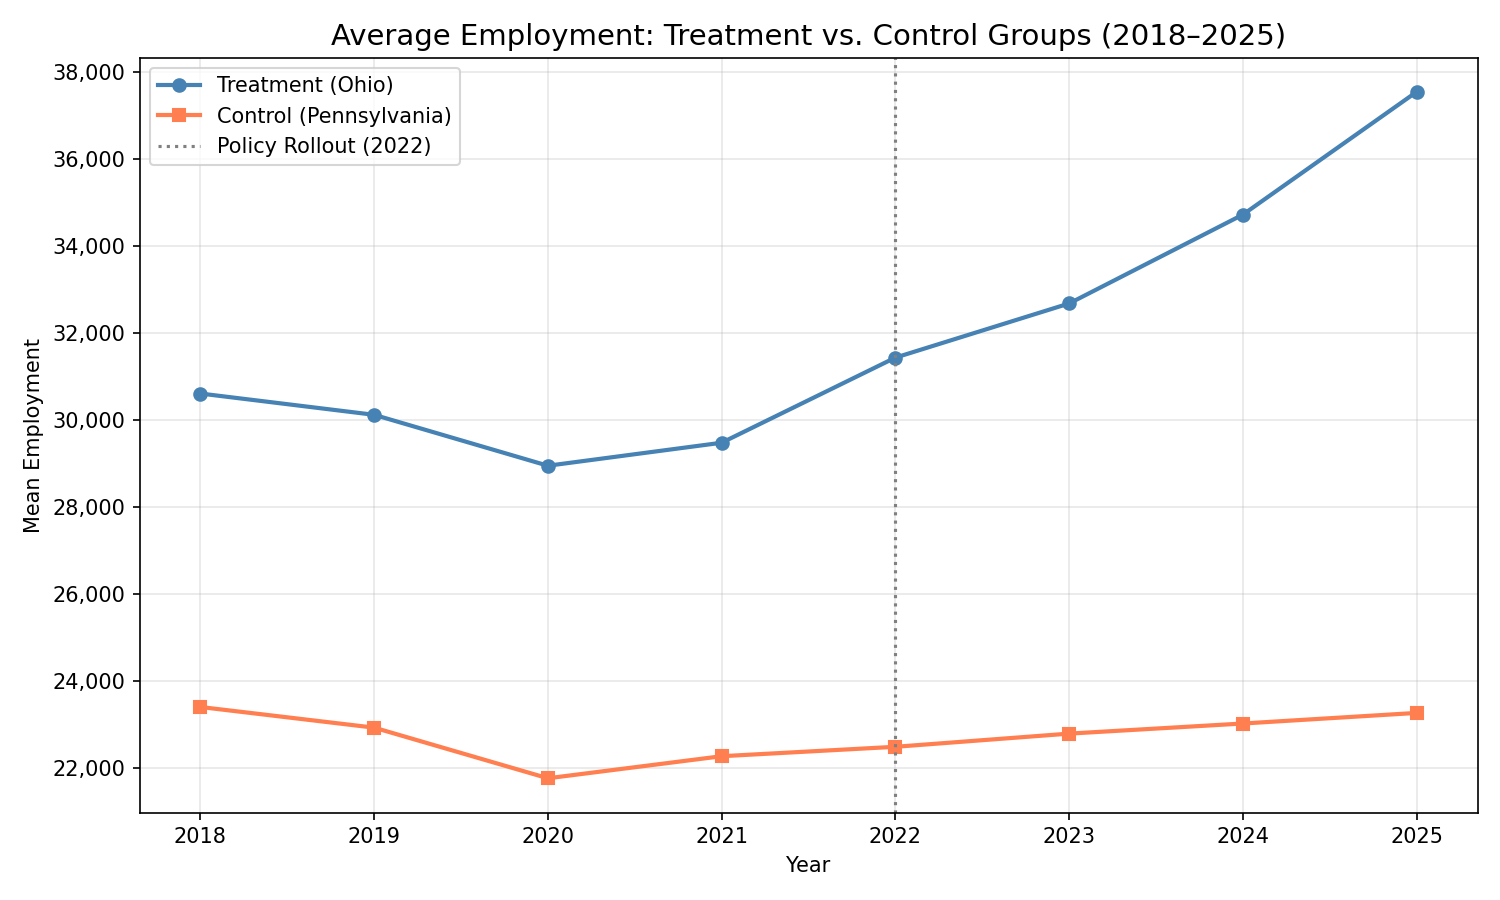
\includegraphics[width=0.85\textwidth]{employment_trends.png}
  \caption{Mean employment for Treatment (Ohio) and Control
    (Pennsylvania) counties, 2018--2025.  The dotted vertical line
    marks the 2022 AI training subsidy rollout.}
  \label{fig:trends}
\end{figure}

% ---------------------------------------------------------------
\section*{Parallel Trends Assumption}
% ---------------------------------------------------------------

Figure~\ref{fig:pt} isolates the pre-treatment window (2018--2021).
Both groups decline at virtually identical rates --- approximately 377
workers per year --- indicating that county-level forces unrelated to
the policy drove common employment dynamics before 2022.  A formal
F-test on the year~$\times$~Treated interaction terms in the pre-period
regression yields $F = 0.13$ ($p = 0.94$), providing statistical
support for parallel pre-treatment trends and validating the
difference-in-differences design.

\begin{figure}[h]
  \centering
  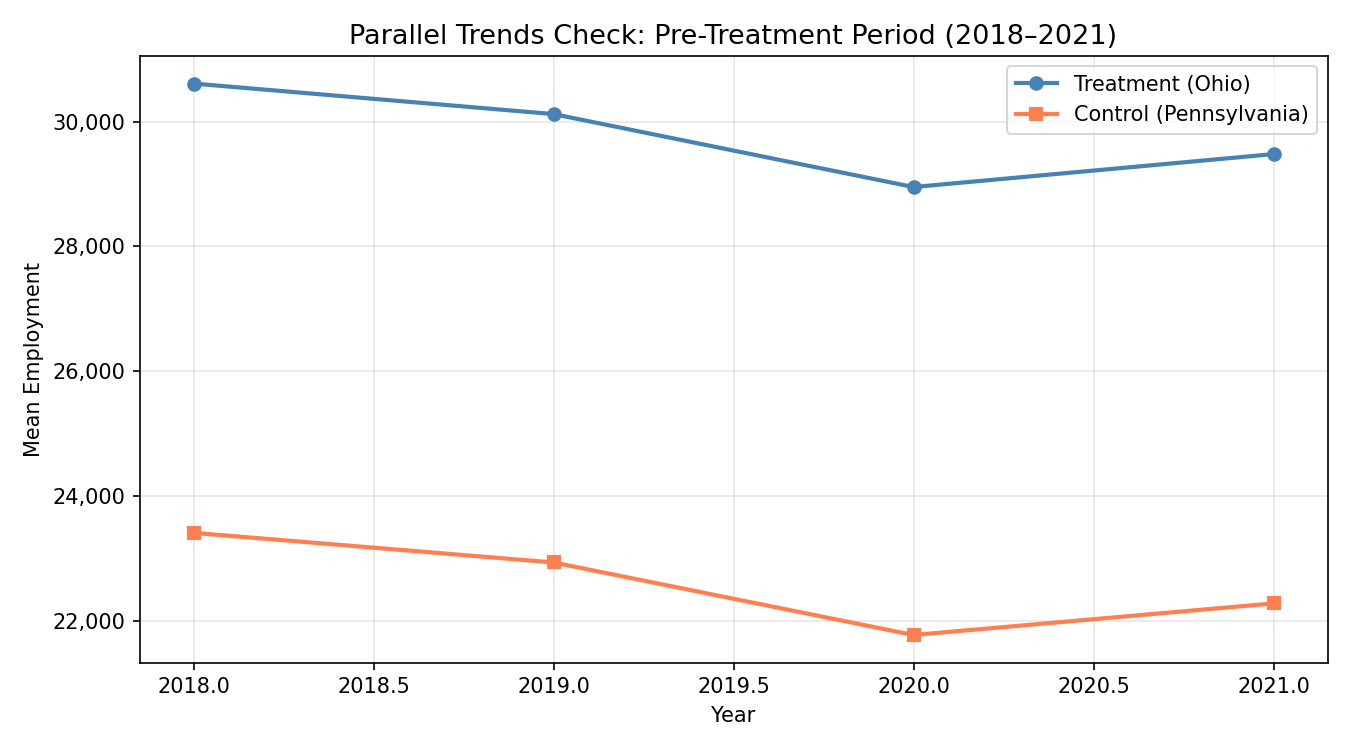
\includegraphics[width=0.80\textwidth]{parallel_trends.png}
  \caption{Pre-treatment employment trends (2018--2021) for Treatment
    and Control groups.  The nearly overlapping slopes support the
    parallel trends assumption required for causal identification.}
  \label{fig:pt}
\end{figure}

% ---------------------------------------------------------------
\section*{Placebo Test}
% ---------------------------------------------------------------

To probe for anticipatory effects, a placebo DID was estimated using
2020 as a fake treatment date restricted to the pre-treatment window
(2018--2021).  The placebo interaction coefficient is $-3.3$ workers
($p = 0.92$), statistically indistinguishable from zero.  This null
result confirms that no pre-treatment divergence existed between groups
and that the post-2022 employment gap is not an artifact of a
pre-existing trend break.

% ---------------------------------------------------------------
\section*{DID Regression Results}
% ---------------------------------------------------------------

The two-way fixed-effects model estimated is
\begin{equation}
  \text{Employment}_{it}
  = \alpha_i + \gamma_t
    + \beta\,\bigl(\text{Treated}_i \times \text{Post}_{t}\bigr)
    + \varepsilon_{it},
\end{equation}
where $\alpha_i$ and $\gamma_t$ are county and year fixed effects,
respectively.  Table~\ref{tab:did} reports the key coefficient.

\begin{table}[h]
  \centering
  \caption{Two-Way Fixed-Effects DID Regression: Effect of AI Training
    Subsidy on Employment}
  \begin{tabular}{lcccc}
    \hline\hline
    Variable
      & Coefficient
      & Std.\ Error
      & $t$-Statistic
      & $p$-Value \\
    \hline
    $\hat{\beta}_{\mathrm{DID}}$
    (Treated $\times$ Post)
      & 4{,}000
      & 480
      & 8.33
      & $<$0.001 \\
    \hline
    \multicolumn{5}{l}{%
      \small\textit{Note}: County and year fixed effects included.
      HC3 heteroskedasticity-robust standard errors.} \\
    \multicolumn{5}{l}{%
      \small Observations: 64.\quad $R^{2} = 0.990$.\quad
      Dependent variable: Employment.} \\
    \hline\hline
  \end{tabular}
  \label{tab:did}
\end{table}

% ---------------------------------------------------------------
\section*{Interpretation}
% ---------------------------------------------------------------

The difference-in-differences estimate indicates that the AI training
subsidy \textbf{increased employment in treated Ohio counties by
approximately 4{,}000 workers per county per year} relative to the
counterfactual trend established by Pennsylvania benchmark counties
($p < 0.001$; 95\% CI: [3{,}059,\;4{,}942]).  Because the parallel
trends assumption is strongly supported --- both visually and through
a statistically insignificant pre-period F-test ($p = 0.94$) --- and
because the placebo test yields a near-zero coefficient ($-3.3$,
$p = 0.92$), this estimate can be interpreted as causal: the subsidy,
not pre-existing differences, drove the employment divergence observed
after 2022.

The validity of the causal identification rests on three pillars
confirmed by the data.  First, pre-treatment trends are virtually
identical across groups, satisfying the parallel counterfactual
assumption.  Second, the placebo test detects no spurious treatment
effect in the pre-period, ruling out anticipatory responses or dynamic
selection into the program.  Third, the two-way fixed-effects structure
absorbs both time-invariant county characteristics (e.g., industrial
composition, geography) and region-invariant time shocks (e.g.,
national business-cycle fluctuations).

Regarding regional labor market dynamics, the results suggest the
subsidy operated primarily through \emph{job creation} rather than
\emph{displacement}.  Control counties --- which reported automation
interest but received no subsidy --- saw employment stagnate near
22{,}600--23{,}300 throughout the panel, implying that automation
without workforce upskilling does not generate net employment gains.
By contrast, treated counties experienced accelerating growth (31{,}400
in 2021 to 37{,}500 in 2025), consistent with a worker-productivity
complementarity in which subsidized training raised human capital
enough to attract new capital investment and expand payrolls rather than
substitute for workers.  The ramp-up pattern --- the annual treatment
effect growing from roughly 1{,}738 workers in 2022 to 7{,}062 by 2025
--- suggests the subsidy's full labor-market impact materialized over a
multi-year horizon, with important implications for how future upskilling
programs should be monitored and evaluated.

\end{document}
